\documentclass[a4paper]{article}
\usepackage{fullpage}
\usepackage[T1]{fontenc}
\usepackage[utf8]{inputenc}
\usepackage{microtype}
\usepackage{amsthm}
\usepackage{amsmath}
\usepackage{hyperref}
\usepackage{lmodern}
\usepackage{enumitem}
\usepackage{tabularx}
\usepackage{ltablex}

\usepackage{listings}
\lstset{basicstyle=\ttfamily, columns=fullflexible,%
  emph={address,bool,bytes32,struct,uint,uint32,uint256},%
  emphstyle={\bfseries}}

% For TikZ diagrams:
\usepackage{pgfplots}
\pgfplotsset{compat=1.11}

\newcommand{\BTC}{BTC}%{\textsc{btc}}
\newcommand{\ETH}{ETH}%{\textsc{eth}}
\newcommand{\hash}[1]{\mathtt{hash}({#1})}
\newcommand{\lotteryhash}[1]{h({#1})}
\newcommand{\randao}{\textsc{randao}}

\title{A~Probabilistic Micropayment Scheme for~Golem}
\author{Golem Team (\texttt{golem@imapp.pl})}

\newtheorem*{dfnt}{Definition}

\newtheorem*{exmp}{Example}
%\setlength{\parskip}{.6em}

\begin{document}
\maketitle

\begin{abstract}
    We consider a~setting where a~payment  is~made by~a~single payer
    to~a~possibly large group of~recipients, each receiving only a~small
    sum in~the~order of~\$$0.01$. For such small sums transaction fees are
    relatively large even if~we consider cryptocurrencies instead of
    bank-based transactions.

    Both payers and~recipients are expected to~repeatedly take part in
    many payments, but subsequent payments of~a~single payer may
    have different groups of~recipients. Also, we
    assume that~payments result from~activities carried out in~a
    decentralized peer-to-peer network, so we would like to~avoid
    solutions relying on~any trusted third party. We cannot therefore use
    existing solutions that~require a~central server or assume that~a
    payer makes a~series of~micropayments to~a~single recipient (Bitcoin
    micropayment channels).

    Instead, we propose a~probabilistic payment scheme in~which only one
    recipient randomly chosen from~a~group of~candidates  is~rewarded in
    a~single payment. Our solution  is~based on~Ethereum and~is~thus
    decentralized and~avoids relying on~a~trusted third party. We describe
    an~Ethereum smart contract implementing a~lottery used to~reward
    recipients and~calculate the~cost of~running it. Depending on~the
    variant of~the~protocol, this cost  is~either proportional to~the0
    logarithm ofthe~number of~recipients or constant. In both cases,
    the~cost of~running a~lottery with~1000~participants is~similar
    to~the~cost of~direct payments to~20~recipients.
\end{abstract}

\section{Introduction}
\label{sec:intro}

    This work  is~part of~research conducted in~the~Golem project. The~aim of~Golem  is~to create a~global prosumer
    market for~computing power, in~which producers may sell spare CPU time of~their personal computers and~consumers
    may acquire resources for~computation-intensive tasks. In technical terms, Golem  is~implemented as a~decentralized
    peer-to-peer network established by~nodes running the~Golem client software. For the~purpose of~this paper
    we assume that~there are two types of~nodes in~the~Golem network: \textbf{requester nodes} that~announce computing
    tasks and~\textbf{compute nodes} that~perform computations (in the~actual implementation nodes may switch between
    both roles).
    A~requester node partitions a~task into~multiple subtasks, specifies payment for~each subtask and~recruits
    a~group of~compute nodes, each of~which downloads and~completes one subtask. This  is~again a~simplifying
    assumption, since~in~principle a~single compute node could complete multiple subtasks.
    Results of~each subtask are sent back to~the~requester node. After the~requester node collects the~results of~all
    subtasks, it performs the~payment step.\footnote{In this scenario we assume that~the~compute nodes do not fail
    and~eventually deliver the~results and~the~requester node  is~willing to~perform the~payment step.
    The~first assumption may be implemented for~example by~ensuring each subtask is~computed by~more than one node
    (in parallel or in~sequence) and~the~second one may be enforced by~a~suitable reputation system for~the~nodes,
    but this  is~outside the~scope of~this paper.} This last step  is~the~main focus of~the~paper.

    In Golem we handle a~variety of~tasks with~different sizes and~decomposable to~a~different degree. In~particular:
    \begin{itemize}
        \item Task partitioning can range from~10 to~$10\;000$ subtasks.
        \item Task value can range from~\$1 to~$\$10\;000$.\marginpar{Czemu nie $\$1$--$\$\infty$?}
        \item Payment for~a~single subtask may be as low as \$0.01 or even \$0.001 for~some types of~tasks.
    \end{itemize}

    The~main requirement for~any payment solution used in~Golem  is~that it should be decentralized and~not depend
    on~any trusted authorities (banks, brokers).

    We should not expect that~after a~payment for~a~subtask  is~made, another payment with~the~same payer and~recipient
    will occur in~a~short time. That is, it may not be possible to~accumulate payments made by~one payer and~transfer
    the~larger sum using a~single transaction. On the~other hand, we may consider methods that~assume recurring
    payments to~a~single payee. That is, a~compute node does not necessarily have to~be paid a~tiny sum for~each
    subtask but instead may be paid larger sums once in~a~while. The~obvious requirement  is~that in~the~long run
    the~node's income should approach the~sum of~subtask values that~this node has computed.

    Thus we are looking for~a~micropayments solution that~handles payments as small as \$0.01 with~transaction fees
    in~the~order of~\$0.0001 per~payment (this does not necessarily mean \$0.0001 per~task which~may group many
    payments). This rules out traditional methods such as bank-based transactions, credit card transactions or PayPal,
    since~transaction fees they incur are in~the~order of~\$0.1, plus a~percentage of~the~transaction value
    (see e.g. \cite{FRS}).

    It seems more promising to~look at~available micropayment schemes based on~digital currencies such
    as Bitcoin \cite{BITCOIN}, which we do in Section~\ref{sec:cryptocurrencies}. In Section~\ref{sec:ethereum} we
    describe Ethereum, a platform for developing decentralized applications, and consider payment methods based
    on Ethereum. In Section~\ref{sec:lottery} we describe the lottery payment scheme, in Section~\ref{sec:costs} 
    we compare costs of various payment schemes based on Ethereum and in Section~\ref{sec:randomness} we discuss some
    details of the lottery implementation. Section~\ref{sec:conclusion} contains concluding remarks. Technical
    details are included in the Appendices~\ref{sec:lottery-description} and~\ref{sec:code}.
    \marginpar{update}

\section{Micropayments schemes for~cryptocurrencies}
\label{sec:cryptocurrencies}    

    We first consider a~naive solution in~which the~requester pays each node participating in~the~computation
    with~a~separate Bitcoin transaction. Although Bitcoin transaction fees are lower than for~bank-based transactions,
    a~transaction smaller than 0.01 \BTC{} ($\sim$ \$2.5 at~the~moment of~this writing) requires a~fee of
    0.0001 \BTC{} ($\sim$ \$0.025) to~discourage "dust" transactions that~bloat the~Bitcoin blockchain \cite{BITFEE}.
    Such~a~fee may thus be be higher than the~transaction value.

    A~Bitcoin transaction may include many outputs, each to~a~different recipient, which~seems a~good match for
    one-to-many payments. We can therefore consider making a~single Bitcoin transaction with~a~separate output
    for~each of~the~participants. In this case, the~flat fee of~0.00001 \BTC{} for~"dust" transactions applies only
    once to~the~whole transaction, so this  is~not an~issue. However, the~size of~the~transaction in~bytes grows with
    each output and~Bitcoin also has fees for~large transactions: the~default charge  is~0.0001 \BTC{} per~1000 bytes.
    Using the~formula for~approximating transaction size from~\cite{BITFEE}:
    \begin{displaymath}
      \texttt{transaction\_size} = 148 * \texttt{number\_of\_inputs} + 34 * \texttt{number\_of\_outputs} + 10
    \end{displaymath}
    we may estimate that~a~transaction with~100 payees will cost at~least \$0.1 and~the~cost will rise as the~coins
    become fragmented and~require a~large number of~inputs. However, as fees in~Bitcoin are~market-based rather than
    hard coded, miners may at~some point start requiring higher fees for~processing transactions \cite{KASKALOGLU}.
    According estimates in \cite{ANDRESEN}, miners should require a~fee of
    at~least 0.0032 \BTC{} ($\sim$ \$0.8) for~including each 1000 bytes in~a~block), to~compensate for~the~fact that
    a~larger block  is~more likely to~be orphaned. Finally, we should point out that receivers of~"dust" payments will
    bear the~cost of~spending the~tiny coins they receive, due to~higher fees for~transactions with~large number of
    inputs. This may discourage potential users from~participating in~Golem. For these reasons, Bitcoin transactions
    with~multiple outputs may be suitable for~tasks with~a~relatively high value (say above~\$10) or small number
    of~participants. For other scenarios a~different payment scheme has to~be used.

    For completeness we also mention Bitcoin micropayment channels (\cite{BITCOINJ}), but this solution does not fit
    our setting as it assumes that~a~payer makes a~series of~micropayments to~one recipient.
    There  is~also a~number of~custom micropayment solutions such as Coinbase Tip \cite{COINTIP}(no longer active),
    or ChangeTip \cite{CHANGETIP} but they rely on~a~trusted third-party that~processes transactions off-chain,
    which~we definitely want to~avoid in~Golem.

\subsection{Probabilistic payments schemes}

    We next turn our attention to~probabilistic payment schemes. The~idea  is~that instead of~paying \$0.01 directly,
    the~payer issues a~"lottery ticket" for~a~lottery with~\$1 prize with~a~$1/100$ chance of~winning. The~expected
    value of~such ticket is~\$0.01. The~advantage is~that on~average only one ticket in~100 will~lead to~an actual
    transaction. Such scheme is~proposed e.g. in~\cite{RIVEST} and~\cite{WHEELER}.
    A~possible implementation of~this scheme may use cryptographic hash functions, for~example SHA-3. First, both
    the~payer and~the~recipient draw (or choose) their numbers $n_P$ and~$n_R$, respectively.
    Both parties initially keep their numbers secret. Then the~recipient reveals $\hash{n_R}$, the hash of $n_R$.
    In the~next step the~payer reveals $\hash{n_P}$. Finally, both parties reveal their numbers (in any order)
    and~use them to~decide if~the~recipient receives the~prize: the~recipient wins if~and~only if~$n_P = n_R \mod N$,
    where $1/N$ is 
    the~probability of~winning. Note that~even if~the~recipient learns $n_P$ before~revealing $n_R$, she cannot change
    her choice of~$n_R$ since~she~committed to~the~original choice by~revealing $\hash{n_R}$ and~it is~considered
    unfeasible to~find another number with~the~same hash.

    Obviously, this probabilistic procedure does not guarantee that~the~Golem node is~fairly remunerated if~it only
    takes part in~a~small number of~tasks. However, as the~number of~tasks increases, the~node's real income from
    lottery rewards will approach the~amount she would get being paid for~each task. For the~requester node the
    situation is~similar, but the~probabilistic effects may be more problematic: suppose a~requester node just
    joined Golem and~now has to~pay for~its first task to~100 other nodes with~tickets giving each receiver
    $1/100$ chance of~winning the~total task value. Now, since~each ticket is~evaluated independently,
    there is~a~37\% chance that~the~requester will not have to~pay anything but also a~substantial 26\% chance that
    at~least two tickets win, and~almost 2\% chance that~at least 4~tickets win. Therefore the~requester should be
    prepared to~pay 4 times more than expected, which~may discourage users from~joining Golem.

    We can modify this scheme to~make it more predictable for~the~requester by~ensuring that~among the~tickets issued
    to~reward the~participants of~a~single task, exactly one ticket is~winning. For example, if~there are 100
    participants then each of~them has $1/100$ chance of~winning, as before, but the~requester has guarantee that
    task value will have to~be paid only once. In other words, after the~task is~completed the~requester will have
    to~organize a~lottery for~the~participants, in~which exactly one participant wins.\footnote{This can be easily
    generalized to~a~constant number $n$ of~winners ($n > 0$) for~a~lottery, each rewarded with~$1/n$ of~the~task
    value.}
    The~drawback of~this approach is~that it requires a~protocol that~involves a~large group of~participants:
    the~payer and~all the~payees.
    Such a~protocol is~more complex than in~a~one-to-one scenario where each lottery ticket is~evaluated separately.

    In the~rest of~this paper we describe and~compare several possible payment schemes (most of~them briefly) in~the
    context of~Ethereum platform.

\section{Ethereum}
\label{sec:ethereum}
    Ethereum \cite{ETHEREUM} is~a~decentralized, blockchain-based crypto currency system, but also a~platform
    for~development of~distributed applications. In Ethereum it is~possible to~implement arbitrary complex rules
    required by~a~payment scheme as \textbf{smart contracts} in~a~high-level programming language (we use Solidity
    \cite{SOLIDITY}, in~this paper).
    This would allow us to~extend payment rules in~the~future, for~example by~including fees for~using
    proprietary software in~a~software-as-a-service model on~compute nodes. Moreover, Ethereum does not suffer from
    coin fragmentation. This makes Ethereum our platform of~choice for~implementation of~micropayment schemes.

    Ethereum has a~notion of~global state which~is~stored in~the~blockchain. This state is, essentially, a~collection
    of~accounts, each with~its unique address and~balance of~\textbf{Ether} (Ethereum's currency). An~account may store some
    data in~a~persistent storage and~may have contract code associated with~it.

    The~global state is~changed by~\textbf{transactions}. Each transaction has a~sender address and~a~recipient address and
    transfers a~specified amount of~Ether between these addresses. If~the~recipient's account is~associated with
    contract code, the~contract is~run as a~result of~the~transaction. The~transaction may carry additional data,
    accessible by~the~contract. A~contract may call another contract, which~may call yet another one, but this chain
    of~execution has to~start with~a~transaction sent by~an~external actor (a~user). A~contract has no way of~calling
    any external service outside Ethereum.

    Contracts are executed by~the~Ethereum Virtual Machine (EVM)\cite{ETHERDEV}. Each EVM instruction consumes certain
    amount of~gas which~reflects a~computational cost of~processing the~instruction by~Ethereum nodes. Gas has to~be
    purchased with~Ether by~the~user who~wishes to~run a~contract. Paying for~gas is~the~analogue of~transaction fees
    in~Bitcoin. Gas price is~market-based: each transaction specifies the~maximum price its sender is~willing to~pay
    for~a gas unit and~miners may prioritize transactions based on~this information. So to~estimate the~cost in~USD
    of~executing a~contract we have to~take into~both the~current average gas price and~the~price of~Ether.
    On the~other hand, in~order to~compare different payment schemes implemented a~Ethereum contracts we can simply
    compare their cost in~gas units.

    Ethereum does not solve all our problems. For example, it provides reliability but not confidentiality, since~all
    data in~Ethereum state is~public (so that~everyone may verify all transactions). This may be an~obstacle for
    implementing certain more complicated payment schemes. For example, a~protocol for~a~lottery may require the
    requesting node and~all compute nodes to~choose secret values that~will be used later to~determine the~lottery
    winner. Those values have to~be produced outside Ethereum, which~gives the~requesting node a~possibility to
    reveal its secret value to~a~chosen compute node making the~lottery unfair.

    Computation model of~Ethereum is~deterministic: the~outcome of~any transaction is~always the~same when it is
    performed in~a~given global state. This limits the~possibility of~generating random values in~Ethereum.
    A common solution is~to rely on~future blockchain data as a~source of~randomness. For example, a~timestamp or
    a~hash of the header of some future block may be used to~seed a~random number generator.\footnote{The hash of a
      future block header depends on future transactions and the output of a proof-of-work algorithm,
      and thus may be treated as a pseudorandom value, see~\cite{WOOD}, Sect.~4, on how it is computed.}

    Ethereum contracts do not have any mechanism to~schedule actions (such as calling another contract or reading a
    timestamp) for~execution at~later time. Therefore any payment scheme using Ethereum will rely on~users willing
    to~perform transactions required by~the~scheme's protocol. In particular, users have to~be online during at
    least some phases of~the~protocol. They also must have enough Ether to~pay for~their transactions, which~may be
    a~problem for~payment protocols that~require not only the~requester node but also compute nodes to~take actions.
    This is~especially severe in~protocols with~many participants, any of~which can stop the~protocol.
    Fortunately, mechanisms for~providing economic incentives for~users to~take actions (deposits, rewards)
    can be easily implemented in~smart contracts.

    \subsection{Infrastructure of Ethereum contracts}
    
    Some of~the~problems listed above~may be solved by~smart contracts provided by~Ethereum community independent of
    Golem. For example, there exist preliminary implementations of \randao{} (RANdom generating Decentralized Autonomous
    Organization) which generate random numbers from users' input. Users are paid for providing inputs with
    money paid by users that consume random numbers. The two \randao{} implementations we are aware of are \cite{RANDAO}
    (compatible with obsolete POC5 version of Ethereum) and \cite{RANDAO2} (more up-to-date).

    Another smart contract that can be useful for our purposes is the Ethereum Alarm Clock \cite{ALARM}
    that allows users to~schedule a~contract call for~a specified future block.
    Users pay for~scheduling their actions and~get paid for~executing other users' actions on~time.

    Both the \textsc{randao} contracts and the Alarm Clock contract rely on a two-sided network effect:
    users on the demand side (requesting random numbers or scheduling message calls) rely on users on the supply side
    (providing input or executing scheduled calls), but users on the supply side will participate only if there is
    enough users on the demand side to provide adequate financial incentive. At this point it is hard to tell whether 
    the userbase for these contracts will be big enough to make them useful.

    In Section~\ref{sec:randomness} we discuss problems with solutions that produce random values based solely on user input,
    such as \textsc{randao}.
    
    In future we may benefit from other solutions developed by~members of~Ethereum community. We also keep in~mind that
    Ethereum still evolves and~new features may appear in~core Ethereum.

    \subsection{Payment schemes in Ethereum}
    \label{sec:ethereum-schemes}

    In this section we consider several payment schemes that can be implemented in~Ethereum:

    \paragraph{Direct transfer (with~batching).}
    This is~a~naive approach in~which the~requesting node makes a~transfer to~each compute node participating in~the~task.
    Simple transfer costs 21 000 gas units for~every user, which~is~about \$0.001 at~the~time of~this writing.\footnote{%
      As of~13 Oct. 2015 average gas price is~$\sim$ 55 Gwei = $5.5 \cdot 10^{-8}$ eth, and~1 eth is $\sim$\$0.6.}
    We also consider a~variant that~uses batching\cite{BUTERIN} to~pack all payments in~one transaction.
    In this case the~cost of~sending ether is~9000 gas units per~node plus the~cost of~sending all data
    to~the~contract (min. 2000 gas per~node). With current gas prices this method gives transaction fees
    below~5\% for~payments of~\$0.01 or more. To handle tasks with~lower payments to~a~single recipient and~to
    account for~fluctuations of~gas price we have to~find a~better method.

    \paragraph{Subaccounts.}
    Another approach is~to create a~smart contract that~keeps in its storage account balances of~every Golem node,
    as a map with user addresses as keys and ether balances as values. 
    To receive payments, users must first register their subaccounts in~the~contract, which is an one time investment
    of approximately $40\;000$ gas.
    In the~payment step, the~payer sends a~list of~recipients and payment values to the~contract, and
    the contract increments each recipient's subaccount balance by the specified payment value. 
    Users can transfer ether from their subaccounts to ``real'' Ethereum accounts at any time, covering the cost of the transfer.
    In this scenario, the~cost of~a~single transaction is~$5\;000$ gas units per~recipient (for modifying the~storage)
    plus the~cost of~sending all data to~the~contract and additional integrity checks (see Section~\ref{sec:costs} for
    more accurate cost estimates).

    \paragraph{Lottery.} 
    This is~a~probabilistic approach in~which the~requester organizes a~lottery in~which only one compute node
    wins. In this scenario the~cost is~generated mainly by~the~size of~data that~needs to~be transferred to
    the~contract. This approach is~described in~Section \ref{sec:lottery} and its cost is estimated in Section~\ref{sec:costs}.

    We also mention two additional payment schemes based on~Ethereum but do not attempt to~estimate their cost:
    
    \paragraph{Micropayment channels.}
    Micropayment channels in~context of~Ethereum are described in~\cite{BUTERIN}. They allow the~user to~send
    transactions off-chain. Unfortunately, as in~the~case of~Bitcoin micropayment channels \cite{BITCOINJ} this
    solution is~designed for~many 1-1 microtransactions between two given parties. The~cost of~opening a~channel
    is~quite large (at least the~cost of~adding 5 new storage fields 20 000 gas each) and~channel endpoints might
    never cooperate again. Additionally, a~micropayment channel requires an~escrow, so if~a~requester has to~open
    many channels the~deposits may sum up to~a~large amount.

    \paragraph{Bank-set approach.}
    Most micropayments protocols for~P2P networks require some sort of~a~centralized institution (bank) that~is
    in~charge of~approving transactions \cite{JAIN}. One idea is~to replace this institution with~a~set of~peers
    (an approach similar to~the~Karma protocol \cite{VISHNUMURTHY}) that~keep track of~transactions and~user accounts.
    The~requester pays the~total amount of~ether for~each task into~one joint Ethereum contract.
    If~a~user wants to~pay out her share from~her account, the~nodes in~the~bank-set vote for~or against the~payout.
    Unfortunately it is~not clear how to~choose bank-set representatives, how Ethereum contract should know
    current representatives, how should they vote and~how to~design a~reward/punishment mechanism
    for~representatives. At the~moment, this solution seems to~be too complicated to~be practical.

\section{Lottery}
\label{sec:lottery}

    Our proposed solution allows the~payer to~avoid making separate transactions to~each of~the~payees. Instead,
    the~whole task value is~paid to~only one payee, chosen randomly. This way, paying for~the~task requires only
    a~small number of~transactions, independent of~the~number of~payees.

    The~idea is~to organize a~lottery for~payees, with~the~reward equal to~the~total value of~the~task. The~lottery
    has only one winner, other participants get nothing. For $i$-th participant the~probability of~winning is~set to
    $v_i/v$, where $v_i$ is~the~payment due to~this participant for~computing a~subtask and~$v$ is~the~value of~the
    whole task. Thus the~expected value of~the~outcome for~this participant is~$v_i$. If~a~participant takes part in
    lotteries for~a large number of~tasks, in~the~long run she may expect the~same income as with~direct payments for
    each subtask.

    Below we describe the~lottery protocol on~a~fairly abstract level. We fill in~the~details in~Section
    \ref{sec:lottery-protocol} and~Appendix \ref{sec:lottery-description}.

    \paragraph{Lottery contract.}
    Lotteries are handled by~a~single Ethereum contract which~stores information about~all the~lotteries that~are in
    progress. Participants (the payer and~payees) send messages to~this contract to~start the~lottery and~claim
    the~reward. The~basic protocol consists of~two types of~messages: \texttt{lotteryInit}, sent by~the~payer to
    establish a~lottery after the~task is~completed, and~\texttt{lotteryWinner}, sent by~any participant
    (presumably the~winner) after the~winner is~determined to~transfer the~reward to~the~winner's account and~end
    the~lottery.

    \paragraph{Starting the~lottery.}
    To start a~new lottery, the~payer creates a~lottery description $L$ and~calculates its hash $\lotteryhash{L}$. The
    description contains a~unique lottery identifier, Ethereum addresses $a_1,\,\ldots,\,a_n$ of~each payee and
    payment values $v_1,\,\ldots,\,v_n$ due to~each payee, possibly together with~some other data. The~payer then
    sends an~\texttt{lotteryInit} message to~the~contract to~announce the~lottery. The~message contains $\lotteryhash{L}$ and
    also transfers the~task value from~the~payer to~the~contract (in Ethereum, each contract is~associated with~an
    account). The~contract stores $\lotteryhash{L}$ in~the~Ethereum persistent storage. Since $L$ contains a~unique lottery
    identifier, $\lotteryhash{L}$ is~also a~unique value and~may be used as a~key when storing and~retrieving various lottery
    data to/from Ethereum persistent storage.

    The~payer also announces the~lottery description $L$ to~the~Golem network, so that~every interested
    node\footnote{ The~lottery description must be sent to~all lottery participants. It can be also sent to~other
    nodes that~are interested in~watching the~lottery contract and~potentially take part in~the~lottery as a
    third party (for example, capture the~hash of~the~deciding block if~the~payer does not do it on~time or reveal
    that~a~node claiming to~be the~winner is~cheating).}
    can verify that~its payment $v_i$ has the~correct value and~check that~$\lotteryhash{L}$ is~indeed written to~the~Ethereum
    storage.

    \paragraph{Determining the~winner.}
    The~winner of~the~lottery can be uniquely determined from~its description $L$ and~some random value $R$ that
    is~not known to~any party at~the~moment the~lottery is~started. We~assume that~$L$ and~the~timestamp $t_0$ of
    the~moment at~which $\lotteryhash{L}$ is~written to~the~Ethereum storage determine another timestamp $t_R$ of~some future
    moment at~which $R$ will be revealed to~everyone. From this moment on, $R$ will also be available to~the~lottery
    contract.

    A~standard way to~implement this rather abstract assumption in~a~blockchain setting is~to use the~hash of~some
    future block as a~random value. When the~lottery is~initialized the~contract increments the~number of~the~current
    Ethereum block by~a~fixed number, determining the~number of~a~deciding block. The~hash of~this future block will
    be used to~determine the~lottery winner. There is~a~problem though with~implementing this simple solution in
    Ethereum (see Section \ref{sec:problem256} for~details).

    \paragraph{Claiming the~reward.}
    Lottery reward may be claimed by~sending a~\texttt{lotteryCheck} message to~the~lottery contract, with~the
    full lottery description $L$. The~contract then calculates $\lotteryhash{L}$ and~checks that~it~exists in~the~storage,
    which~indicates that~the~lottery has started but the~reward has not been claimed yet.
    If~$t_R$ has elapsed and~$R$ is~available, the~contract computes the~winner's address from~$L$ and~$R$ and
    transfers the~reward from~the~contract's account to~the~winner. At this point, the~contract removes $\lotteryhash{L}$
    from~the~storage.

    The~problem with~the~basic protocol is~that the~size of~$L$ is~proportional to~the~number of~payees and~whoever
    sends the~\texttt{lotteryCheck} message has to~pay for~sending $L$ and~processing it by~the~contract.
    Taking into~account that~sending a~byte of~data in~a~message costs 68 gas units we estimate that~sending and
    processing the~message will require at~least 2000 gas units per~payee. This would defeat the~whole lottery
    approach, which~was proposed in~order to~avoid paying transaction fees proportional to~the~number of~payees.

    Fortunately, in~order to~verify that~$a_i$ is~the~winner the~contract does not need to~examine whole $L$.
    If~the~list of~payees with~their payment values is~stored in~a~data structure called \textbf{Merkle tree} then it~is
    enough to~send and~examine an~amount of~data proportional to~the~logarithm of~the~number of~payees
    (see Appendix \ref{sec:lottery-description} for~details). Therefore instead of~sending
    full lottery description with~\texttt{lotteryCheck} we can send the~address $a_i$ and~just enough
    data to verify that this is the winner's address.

\subsection{Optimistic approach}\label{sec:optimistic}
    If~there is~a~lot of~payees, the~cost of~\texttt{lotteryCheck} may still be high even when only a~part of~the
    lottery description is~required to~compute the~winner. We propose an~extension of~the~basic protocol that~allows
    the~parties to~avoid sending the~\texttt{lotteryCheck} message altogether. Instead, a~payee can claim to~be the
    winner by~sending a~new \texttt{lotteryWinner} message containing only $\lotteryhash{L}$. The~contract cannot verify the
    claim and~only checks that~$\lotteryhash{L}$ exists in~the~storage. Then the~contract stores additional data along with
    $\lotteryhash{L}$, namely the~address $a_i$ of~the~claimed winner and~a~computed deadline timestamp $t_d$ which~determines
    when the~reward may be paid to~$a_i$.

    \paragraph{Claim verification.}
    Until the~deadline $t_d$ elapses anyone can reveal the~true winner by~sending a~\texttt{lotteryCheck} message with
    winner address $a_i$ and~enough data to~validate it. Sending a~\texttt{lotteryCheck} message after a
    \texttt{lotteryWinner} message should only happen if~the~payee that~claimed to~be the~winner is~caught cheating,
    which~we hope will occur rarely (hence the~name "optimistic approach"). To encourage peers to~reveal cheaters,
    and~to punish dishonest participants, we provide a~mechanism of~deposits. A~payee sending the~\texttt{lotteryWinner}
    message must transfer a~deposit which~is~paid back if~no one protests before~the~deadline elapses.
    This deposit is~a~reward for~proving that~the~payee claiming to~be the~winner is~cheating.

    \paragraph{Paying out the~reward.}
    After the~deadline $t_d$ elapses, anyone may send a~message \texttt{lotteryPayout} with~$\lotteryhash{L}$ as the~argument.
    If~$\lotteryhash{L}$ exists in~the~storage and~the~address of~the~payee claiming to~be the~winner is~set, the~reward is
    transferred to~this address and~the~lottery data is~erased from~the~storage.

    Under the~assumption that~all participants are honest, the~cost of~a~lottery is~constant, independent of~the~number
    of~payees.
    An~important property of~the~protocol described above~is~that after the~random value is~revealed, the~payee who
    determines to~be the~winner may calculate the~cost of~a~\texttt{lotteryCheck} message and~decide whether to~perform
    the~basic protocol by~sending \texttt{lotteryCheck} and~obtain the~reward immediately (modulo the~time required by
    the~Ethereum network to~confirm the~transaction), or to~follow the~extended protocol by~sending the
    \texttt{lotteryWinner} with~a~deposit, wait until~the~deadline elapses and~send the~\texttt{lotteryPayout} message
    to~get the~lottery reward.
\subsection{The~problem of~256 past~blocks}
    \label{sec:problem256}
    Recall that~we planned to~use the~hash of~a~future Ethereum block (deciding block) to~determine who~wins
    the~lottery. More precisely, we assume that~when the~lottery is~started the~contract computes the~number
    of~the~deciding block and~stores this number together with~other lottery data. Later on,
    when~a~\texttt{lotteryCheck} is~sent the~contract checks if~a~block with~the~required number has already been
    produced and~if so, uses its hash to~calculate who~is~the~winner. Now, a~problem with~this approach is~that in
    Ethereum, contracts can only access hashes of~the~last 256 blocks. Since a~block is~created roughly each 15
    seconds, this gives us only about~an~hour during which~the~hash value is~directly available from~the~contract.
    There is~no possibility of~scheduling a~message for~sending at~a~later time in~Ethereum, other than relying on
    a~third-party contract (for example Alarm Clock Contract \cite{ALARM}), so during this hour some party has
    to~explicitly send either a~\texttt{lotteryCheck} message that~will use the~hash value to~compute the~winner,
    or some other message that~will prompt the~contract to~store the~hash value for~later use.

    \paragraph{Capturing the~hash of~the~deciding block.}

    To address this issue we extend the~protocol with a~\texttt{lotteryCaptureHash} message the~result of~which is~to
    store the~hash of~the~deciding block. To~encourage sending this message soon after the~deciding block is~generated
    we require that~the~sender of~a~\texttt{lotteryInit} message deposits an~additional amount on~the~contract's
    account, together with~the~lottery reward. The~deposit is~returned to~the~payer if~the~payer sends a
    \texttt{lotteryCaptureHash} message within 128 blocks after the~deciding block is~generated.
    Between 128 and~256 blocks after the~deciding block anyone may send this message and~claim the~payer's deposit.

    As a~last resort, if~the~hash of~the~deciding block is~not stored and~at least 256 more blocks are generated,
    a~\texttt{lotteryCaptureHash} message will store the~hash of~the~unique available block with~the~number congruent
    modulo 256 to~the~number of~the~original deciding block. In this case, the~payer's deposit will remain in~the
    contract's account. Thus instead of~trying to~retrieve the~lost hash we allow the~winner to~be changed.

    If~we could overcome the~problem of~256 blocks then a~payer deposit and~\texttt{lotteryCaptureHash} message would
    be pointless and~protocol would become simpler. An~alternative solution would be to~use a~separate contract
    for~providing hashes of~past blocks. See Section \ref{sec:randomness} for~more remarks on~alternative sources
    of~randomness.
\subsection{Lottery agents}
    We have to~account for~a situation when the~lottery winner goes offline for~a longer period of~time and~is
    unable to~claim the~reward or simply does not want or cannot pay for~sending a~\texttt{lotteryCheck} or
    \texttt{lotteryWinner} message. In such cases a~third party may serve as \textbf{lottery agent} sending messages
    instead of~the~winner while keeping part of~the~reward. In particular, after a~fixed amount of~time elapses
    since~the~time when the~random value $R$ is~revealed (the time when the~deciding block is~produced) and~nobody has
    claimed to~be a~winner, anyone may send the~\texttt{lotteryCheck} message which~will transfer part of~the~reward,
    say 10\%, to~the~sender of~the~message and~the~rest to~the~winner, and~will erase the~contract from~Ethereum
    storage.

\section{Lottery Protocol Specification}
\label{sec:lottery-protocol}
    The~lottery contract is~implemented in~Solidity \cite{SOLIDITY}, a~high-level language compiled to~machine code of
    the~Ethereum Virtual Machine\cite{ETHERDEV}. A~contract in~Solidity consists of~a~number of~functions, each
    function is~a~entry point to~the~contract code. A message sent to the contract identifies a function to be called
    and specifies values of the function's arguments. Below we list Solidity functions that correspond to messages
    in the~lottery protocol. The~following data types of~arguments are used:
    \begin{itemize}
        \item \texttt{uint} (an alias for~\texttt{uint256}) is~the~type of~256 bit unsigned integers,
        \item \texttt{bytes32} is~the~type of~fixed-size arrays of~32 bytes,
        \item \texttt{address} is~the~type of~160 bit Ethereum addresses.
    \end{itemize}
    In all the~functions, the~first parameter (\texttt{bytes32 lotteryHash}) is~used to~specify the~lottery on~which
    the~function operates. Money is~denominated in~wei ($1$ wei = $10^{-18}$ ether) and~represented as \texttt{uint} values.

    \paragraph{Contract functions.} The following functions of the lottery contract can be invoked by users.
    The cost of each function is estimated based on the contract code in Appendix~\ref{sec:code}.

    \begin{itemize}
        \item \verb!function lotteryInit(bytes32 lotteryHash)!

            The~sender Initializes a~lottery. Lottery value is~transferred to~the~lottery contract and~a~structure
            with~lottery data is~created in~the~storage. \texttt{lotteryHash} is~the~value used as a~key to~retrieve
            lottery data from~the~contract storage (see Appendix \ref{sec:lottery-description} for~information on how it
            is~computed). 

            Estimated cost: $65\;000$ gas.

        \item \verb!function lotteryWinner(bytes32 lotteryHash)!

            The~sender claims to~be the~winner.

            Estimated cost: $30\;000$ gas.

        \item \verb!function lotteryCaptureHash(bytes32 lotteryHash)!

            The~message saves the~hash of~maturity block if~it is~possible. The~payer should send this message
            within $128$~blocks since~maturity in~order to~get back the~payer deposit.
            Later, but within $256$~blocks, anyone else can send this message and~get the~payer deposit as a~reward.

            Estimated cost: $35\;000$ gas.
            
        \item{} \verb!function lotteryCheck(bytes32 lotteryHash, uint256 uid, address winner,!\\
                \verb!                      uint32 rangeStart, uint32 rangeLength,!\\
                \verb!                      bool[] path, bytes32[] values)!
          
            The~sender specifies an~address and~the~data required to~verify that~it is~the~winner's address.
            If~the~address is~verified, the~reward is~transferred and~the~lottery data is~erased from~the~storage.

            Estimated cost: $40\;000 + 2\;700 \cdot \log_2(N)$ gas.

        \item \verb!function lotteryPayout(bytes32 lotteryHash)!

            The~sender wants to~receive her claimed reward after deadline elapsed. Transfers the~reward and~erases
            lottery data from~the~storage.

            Estimated cost: $30\;000$ gas.

    \end{itemize}

    \paragraph{LotteryData struct.}
    For every lottery that~is~in progress the~following Solidity structure is~stored in~the~Ethereum storage:

    \begin{lstlisting}
    struct LotteryData {
        uint value;
        uint maturity;
        uint deadline;
        uint randVal;
        address payer;
        address winner;
    }
    \end{lstlisting}
%
    The~meaning of~the~fields is~as follows:
    \begin{itemize}
        \item \texttt{value} is~the~lottery reward (in wei),
        \item \texttt{maturity} is~the~number of~the~deciding block, % (denoted by $t_R$ in Sec.~\ref{sec:lottery}),
        \item \texttt{deadline} is~the~timestamp at~which the~user that~claimed to~be the~winner may collect
            the~reward, % ($t_d$ in Sec.~\ref{sec:lottery}),
        \item \texttt{randVal} is~the~random value determined from~the~hash of~the~deciding block, % ($R$ in Sec.~\ref{sec:lottery}),
        \item \texttt{payer} is~the~address of~the~user that~created the~lottery,
        \item \texttt{winner} is~the~address of~the~user that~claimed to~be the~winner.
    \end{itemize}
    %
    The~contract will also have an~\texttt{uint} variable \texttt{golemDeposit} which~will store
    the~total amount collected in~the~contract from~commissions and~lost deposits. This amount will be eventually
    redeemed by~equity token holders (all Golem application owners).

    The~syntax of~Solidity is~similar to~JavaScript. In particular, if~lotteries is~a~mapping of~uints to~structs of~type LotteryData then the~statement
    \begin{quote}
      \verb!lotteries[lotteryHash].deadline = t!
    \end{quote}
    will update the~field \texttt{deadline} in~the~\texttt{LotteryData} struct for~a~lottery with~hash
    \texttt{lotteryHash}. One difference from~JavaScript is~that in~Solidity a~\texttt{mapping} is~a~total
    function, in~particular \texttt{lotteries} initially maps all possible key values to
    a~\texttt{LotteryData} struct with~all fields initialized to~0. To check if~a~lottery data has been initialized
    we will check if~\texttt{lotteries[lotteryHash].value} is~nonzero.


\paragraph{Protocol.}
    In the~description of~messages below~the~semantics of~the~\textbf{Preconditions} and~\textbf{Effects} clauses is
    that~if all the~conditions specified in~\textbf{Preconditions} are satisfied then the~contract's state is~changed
    as described in~\textbf{Effects}. Otherwise, the~message has no effect on~the~state of~the~contract.
    \begin{enumerate}
        \item The~payer negotiates payment with~every payee independently. Let $v_i$ be the~amount that~$i$-th payee
            expects after this step and~let $a_i$ be the~address of~the~$i$-th payee.
        \item The~payer calculates the~transaction value $v = \sum_i v_i$, calculates the~probability of~winning
            for~each payee and~composes a~lottery description $L$ containing these data (see Section
            \ref{sec:lottery-description} for~details). The~payer then sends $L$ to~every payee. The~payees check that~$L$
            is~correct. In particular, they may verify that~the~expected lottery reward for~the~$i$-th payee is~equal
            to~$v_i$.
        \item The~payer sends a~\texttt{lotteryInit} message to~the~contract with~the~lottery hash $\lotteryhash{L}$ as the
          argument. The~lottery hash can be calculated by~anyone who~knows $L$ and~is~used as a~key for
          storing/retrieving lottery data throughout the~protocol (see Section \ref{sec:lottery-description} for~information
          how $\lotteryhash{L}$ is computed).\\
            \textbf{Preconditions}: no \texttt{LotteryData} struct is~associated with~$\lotteryhash{L}$ in~the~contract's
            storage. This is~equivalent to~the~condition
            \begin{quote}
	      \verb!lotteries[lotteryHash].value == 0!
            \end{quote}
            %
            \textbf{Effects}: The~message transfers the~lottery value $v$ and~the~payer deposit (additional 10\%
            of~$v$) to~the~contract and~stores the~\texttt{LotteryData} struct for~the~new lottery. The~field value
            is~set to~$10/11$ of~the~value transferred by~the~\texttt{message} and~and the~remaining $1/11$ of~this value
            is~treated. Field \texttt{maturity} is~initialized with~argument $m$ and~\texttt{payer} is~initialized with
            the~sender's address. The~remaining fields are initialized with~zeros.
            \begin{quote}
              \verb!lotteries[lotteryHash] = LotteryData(value, block.number + maturity,!\\
              \verb!                                     0, 0, msg.sender, 0)!
            \end{quote}
            At this point any payee can calculate the~hash of~the~lottery on~its own and~can verify if~it exists in
            the~contract's storage. It can be done by~querying the~(locally available) Ethereum state.
        \item Anyone (not only a~payer) can send a~\texttt{lotteryCaptureHash} message with~argument $\lotteryhash{L}$ to~write
            the~hash of~the~deciding block as the~lottery seed.\\
            \textbf{Preconditions}:
            \begin{enumerate}
                \item The~value field of~the~\texttt{LotteryData} for~the~lottery has been set (meaning that~the
                lottery has been initialized but not finalized yet).
                \begin{quote}
                  \verb|lotteries[lotteryHash].value != 0|
                \end{quote}
                \item The~lottery \texttt{randVal} has not been set yet.
                  \begin{quote}
	            \verb!lotteries[lotteryHash].randVal == 0!
	          \end{quote}
                \item The~maturity has elapsed (the stored maturity number is~less than current pending block number).
                  \begin{quote}
                    \verb!lotteries[lotteryHash].maturity < block.number!
                  \end{quote}
	        \end{enumerate}
        \textbf{Effects}:
        \begin{enumerate}
            \item  If~the~difference of~the~current block number and~maturity is~not greater than 128 then the~hash of
                the~deciding block is~written as the~\texttt{randVal} and~the~payer deposit is~transferred to~the~payer.
                \begin{quote}
                  \verb!lottery.randVal = random(lottery.maturity);!\\
                  \verb!lottery.payer.send(calculatePayerDeposit(lottery.value));!
                \end{quote}
            \item If~the~difference of~the~current block number and~maturity is~greater than 128 but not greater than
                256 then  the~hash of~the~deciding block is~written as the~\texttt{randVal} the~payer deposit
                is~transferred to~the~message sender.
                \begin{quote}
                  \verb!lottery.randVal = random(lottery.maturity);!\\
                  \verb!msg.sender.send(calculatePayerDeposit(lottery.value));!
                \end{quote}
            \item If~the~difference of~the~current block and~maturity is~greater than 256 then the~hash of~the~block
            with~number maturity$+k \cdot 256$, where $k$ is~the~greatest possible integer, is~written to~the~contract
            as the~\texttt{randVal} and~the~payer deposit remains in~the~contract (a contract owner gets it).
            \begin{quote}
              \verb!lottery.randVal = random(changeMaturity(lottery.maturity));!\\
	      \verb!golemDeposit += calculatePayerDeposit(lottery.value);!
	    \end{quote}
        \end{enumerate}

        \item Anyone (not only a~payee) can send a~\texttt{lotteryWinner} message to~claim that~she is~the~winner.
            The~message contains the~lottery hash and~requires to~transfer a~winner deposit.\\
            \textbf{Preconditions}:
            \begin{enumerate}
            \item The~maturity stored for~the~lottery has been set.
              \begin{quote}
                \verb|lotteries[lotteryHash].maturity != 0|
              \end{quote}
            \item The~maturity has elapsed.
              \begin{quote}
		\verb|lotteries[lotteryHash].maturity < block.number|
	      \end{quote}
            \item Nobody has claimed to~be the~winner yet.
              \begin{quote}
                \verb|lotteries[lotteryHash].winner == 0|
              \end{quote}
            \end{enumerate}
            \textbf{Effects}:
            \begin{enumerate}
            \item The~contract sets the~claimed winner to~the~sender's address and~sets deadline.
              \begin{quote}
                \verb|lottery.winner = msg.sender;|\\
                \verb|lottery.deadline = now + deadline;|
              \end{quote}
            \item If~the~\texttt{randVal} is~not set than calls \texttt{lotteryCaptureHash} message.
              \begin{quote}
                \verb|lotteryCaptureHash(lotteryHash)|
              \end{quote}
            \end{enumerate}
            
        \item Anyone (not only a~payee or the~payer) can send a~\texttt{lotteryCheck} message. The~message contains
            the~lottery hash and~the~data required to~compute the~winner (see Section \ref{sec:lottery-verification}
            for~details).\\
            \textbf{Preconditions:}
            \begin{enumerate}
            \item The~maturity stored for~the~lottery has been set
              \begin{quote}
                \verb|lotteries[lotteryHash].maturity != 0|
              \end{quote}
            \item The~maturity has elapsed.
	      \begin{quote}
                \verb|lotteries[lotteryHash].maturity < block.number|
              \end{quote}
	    \end{enumerate}
	    \textbf{Effects:}
	    \begin{enumerate}
            \item If~the~\texttt{randVal} is~not set than call \texttt{lotteryCaptureHash} message.
              \begin{quote}
                \verb|lotteryCaptureHash(lotteryHash)|
              \end{quote}
            \item If~28800 blocks has been added to~the~blockchain after the~deciding block (this would take
              approx. 5 days) then 10\% of~the~transaction value $v$ is~transferred to~the~sender (which is~treated
              as a~lottery agent) and~the~transaction value is~reduced to~90\% of~its previous value.
              \begin{quote}
                \verb|msg.sender.send(countAgentProvision(lottery.value));|
              \end{quote}
            \item If~the~winner field is~set to~0 in~the~lottery data than the~transaction value is~sent to~the
              winner.
              \begin{quote}
                \verb|winner.send(lottery.value);|
              \end{quote}
            \item If~the~winner field is~equal to~the~winner address then the~transaction value and~the~winner
              deposit are transferred to~the~winner.
              \begin{quote}
		\verb|winner.send(lottery.value + calculateWinnerDeposit(lottery.value));|
	      \end{quote}
	    \item If~the~winner field is~not equal to~the~winner address then the~transaction value is
	      transferred to~the~winner, winner deposit is~transferred to~the~sender.
	      \begin{quote}
		\verb|msg.sender.send(calculateWinnerDespoit(lottery.value));|
              \end{quote}
            \item The~lottery is~erased from~the~contract.
              \begin{quote}
                \verb|delete lotteries[lotteryHash]|
              \end{quote}
            \end{enumerate}
          \item Anyone can send a~\texttt{lotteryPayout} message to~the~contract. The~message contains the~lottery hash.\\
            \textbf{Preconditions:}
            \begin{enumerate}
            \item The~deadline has elapsed.
              \begin{quote}
		\verb|lotteries[lotteryHash].deadline < now|
              \end{quote}
            \item Somebody has claimed to~be a~winner (winner isn't set to~zero).
              \begin{quote}
                \verb|lotteries[lotteryHash].winner != 0|
              \end{quote}
            \end{enumerate}
            \textbf{Effects:}
            \begin{enumerate}
            \item The~transaction value and~the~deposit are transferred to~the~claimed winner.
              \begin{quote}
		\verb|lottery.winner.send(lottery.value + calculateWinnerDeposit(lottery.value))|
	      \end{quote}
            \item Transaction is~completed and~the~lottery data is~erased from~the~contract.
              \begin{quote}
                \verb|delete lotteries[lotteryHash]|
              \end{quote}
            \end{enumerate}
    \end{enumerate}

    \paragraph{Storage size optimization.}
    In the final version of the contract we optimize the storage size
    of \verb!LotteryData!. The values of both maturity and deadline
    can be kept in the same field of the struct, as they have the same
    size and are never required at the same time: deadline is only set
    when someone sends \verb!lotteryWinner! message and at this point
    maturity is no longer needed.
    %
    Moreover, we can keep payer address and winner address in the same
    field. Payer address is only required for returning payer
    deposit. When winner address is being set, the random value must
    already be fixed and the deposit is already returned or lost. This
    allows us to limit size of final structure from 6 fields to 4.
    
    Additionally, we can pack whole struct in two 256-bit
    words. Lottery value will be kept in one word and all the other
    values can be packed in one storage word: 8 bytes are enough for
    block numbers in maturity/deadline field, 4 bytes to keep random
    value (see remarks in Appendix~\ref{sec:lottery-description}) and
    20 bytes to keep payer/winner address.  Writing a 256-bit word to
    the storage costs $20\;000$ gas, so using 2 words for \verb!LotteryData!
    instead of 5 allows us to cut the cost of \verb!initLottery! in half.

    When estimating gas use (and cost in ethers) of the messages we
    assume the optimization has been done, even though for simplicity
    in Appendix~\ref{sec:code} we show contract code before optimization.
    
\section{Cost comparison}
\label{sec:costs}
    In this section we compare transaction fees in payment schemes
    considered in Section~\ref{sec:ethereum-schemes} for varying
    number of users. For each scheme we estimate the total amount of
    gas required to pay for a single task.\marginpar{cost for whom?}
    For calculating the required amount of gas we take into account the
    following operations:
    \begin{itemize}
    \item sending a message to a contract ($21\;000$ gas),
    \item tranfering data to a contract ($68$ gas for one nonzero byte),
    \item transferring ether to other account in a contract ($9\;000$ gas),
    \item writing new storage entry ($20\;000$ gas for each nonzero 256-bit word),
    \item modifying existing storage entry ($5\;000$ gas for each 256-bit word),
    \item computing SHA-3 hash ($222$ gas for hashing a 256-bit word).
      \marginpar{Może być tak (new entry/existing entry)?}
    \end{itemize}

    Other operations have negligible cost. The costs are summarized in Table~\ref{table:costs}
    and shown in graphical form in Figure~\ref{fig:costs}.
    \begin{table}
      \begin{tabular}{p{9em}p{4em}p{7em}p{6em}p{6em}p{6em}}
        \hline
        Method & Constant cost & Cost per user& Cost for~10 users & Cost for~100 users & Cost for~1000 users \\ \hline
        Batched transfers   & 21 000  & 11 000 & 130 000 & 1.1 mln & 11.2 mln \\ %\hline
        Subaccounts         & 21 000  &  8 000 & 100 000 & 840 000 &  8.2 mln \\ %\hline
        Lottery (check)     & 140 000 & $\log_2(n)/n \cdot 2700 $ & 150 000 & 155 000 & 165 000 \\ %\hline
        Lottery (optimistic)& 155 000 & 0 & 155 000 & 155 000 & 155 000 \\ \hline
      \end{tabular}
      \caption{Transaction costs in gas for different payment methods.}
      \label{table:costs}
    \end{table}
    \begin{figure}
      \centering
      \includegraphics[scale=1.0]{payments.pdf}
      \caption{Transaction costs for~different payment methods, in graphical form.}
      \label{fig:costs}
    \end{figure}

    Note that when using direct transfers, only the payer bears the
    transaction costs, while other payment methods also incur costs
    for the recipients: in the subaccounts approach recipients pay for
    transferring ether to their accounts and in the lottery approach
    the winner pays for claiming the reward. To facilitate comparison
    between payment methods we assume that the recipients will
    negotiate higher payments to compensate for additional costs and
    thus effectively all transaction costs will be covered by the payer.\marginpar{Czy to ma sens?}

    In the subaccounts approach the recipients decide when to transfer
    ether from their subaccounts managed by the payment contract. Each
    such transfer requires approximately $35\;000$ gas and we assume that
    users on average delay the transfer long enough that the transaction
    fee for a single task does not exceed $1\;000$ gas. Thus per-user cost
    in the subaccount approach is estimated at $8\;000$ gas ($2\;000$ for passing
    the recipient's address and payment value to the contract, $5\;000$ for
    updating the balance and $1\;000$ as the amortized cost of transferring ether
    from the subaccount).

    In both variants of the lottery approach, payer fees are constant
    ($\sim 100$k gas for initializing the lottery and capturing the
    hash of the deciding block) independent on the number of
    participants. The winner is free to decide which variant to choose.
    If the number of participants does not exceed $128$ then sending \verb!lotteryCheck!
    is the cheapest option, for larger number of participants the optimistic
    variant has lower fees. There is however a tradeoff: optimistic approach has
    lower transaction fees but the winner has to wait approximately 24 hours after
    sending the \verb!lotteryWinner! message to collect the reward. 

    Note also that for a task with $1\;000$ participants it is less
    expensive to run 10 lotteries (one for each 100 participants and
    with $1 / 100$ chance of winning $1 / 10$ of the total task value)
    than to pay using batched transfers or subaccounts.
    
    \subsection{Costs in fiat currency}
    We may also give corresponding costs in USD, using the
    gas/\ETH{} and \ETH{}/USD rates at the~time of this~writing.%
    \footnote{As of 13 Oct.\ 2015, average
      gas price is approximately $5.5 \cdot 10^{-8}$ \ETH{} and one
      ether costs approximately \$0.6}%
    As the \ETH{}/USD rate changes quickly (and will probably do so in
    the future, taking into account the history of Bitcoin price),
    transaction costs in any fiat currency should be taken as very
    rough estimates, so we round the values up to the nearest power of ten.
    In this~approximation Table~\ref{table:costs} collapses to just two rows,
    as shown in Table~\ref{table:costs-usd}.
       
    \begin{table}
      \centering ~\\~\\  % ugly hack to force more space between table and preceeding figure
      \begin{tabular}{lrrr} 
        \hline
        Method              & Cost for~10 users & Cost for~100 users & Cost for~1000 users \\ \hline
        Batched transfers/subaccounts  & ~ \$0.01          & ~ \$0.1            & ~ \$1    \\ %\hline
        Lottery (either variant)       & ~ \$0.01          & ~ \$0.01           & ~ \$0.01 \\ \hline
      \end{tabular}
      \caption{Transaction costs in USD for different payment methods, order-of-magnitude estimates.}
      \label{table:costs-usd}
    \end{table}

    \subsection{So, which payment method should I use to pay for my task?}
    Assumming the payer wants to keep transaction fees on the level of $1\%$,
    direct transfers or subaccounts are appropriate for tasks in which
    each participant is to be paid at least $\$0.1$, for example a
    task worth \$1 computed by $10$ users of a task worth $\$1\;000$
    computed by $10\;000$ users.

    A lottery must be used for tasks in which participants are to be paid less than $\$0.1$.
    It may also be used if there are at least 20 participants and the payer wants to
    minimize transaction fees even at the cost of using a more complex and probabilistic payment method.
    Note that the constant cost of the lottery approach is low enough to make it suitable for tasks with
    total value of $\$1$, which is the minimum task value Golem will need to handle (see Section~\ref{sec:intro}).

    When comparing costs of various methods we should take into account another factor besides gas requirements.
    Namely, if given a choice users will probably prefer to participate in tasks for which payment is made with
    deterministic methods and the outcome is more predictable. For similar reasons, lotteries with less paricipants
    will be preferred, as they are more likely to provide a reward.
    If the compute nodes are in short supply, lottery rewards will have to be higher than task value paid with
    batched transfers or subaccounts method, to encourage nodes to participate. This may drastically limit the
    applicability of the lottery method.

\section{Source of~randomness for~the~lottery implementation}
\label{sec:randomness}
    In our lottery implementation we use the~hash of~a~future block as the~source of~randomness. This solution has
    two drawbacks. First, there is~a~risk that~the~random value may be manipulated by~Ethereum miners. That is,
    a~miner may decide whether to~publish a~newly found block after looking at~the~block hash and~calculating
    the~winning address. Clearly, if~the~lottery reward is~small compared to~the~reward for~finding a~new block
    then it is~not profitable to~withhold a~block to~change the~odds of~winning a~lottery. Thus one way to~circumvent
    this problem is~to limit the~maximum lottery reward and~in~case the~task value exceeds this limit, split payees
    into~several groups and~organize a~separate lottery for~each group, with~a~fraction of~the~task value as the
    reward.

    The~second problem is~due to~the~fact that~only the~hashes of~past 256 blocks are available in~the~contract
    so we have to~complicate the~protocol and~introduce the~mechanism of~deposits to~encourage the~participants
    to~capture the~hash of~the~deciding block.

    Let us consider some alternatives to~using block hashes as the~source of~randomness.

    \subsection{RANDAO approach}
    Let us consider a~protocol in~which the~winner is~determined using only data provided by~a~group of~participants,
    in~a~peer-to-peer environment, without using any external sources (including hashes of~future block) and~without
    relying on~any trusted third party. That is, each participant reveals a~piece of~data and~once all data is~public
    the~winner is~determined in~a~provable way.

    The~protocol needs to~deal with~situations in~which some participants fail to~reveal their data. This may be due
    to~communication failure or may be done on~purpose. Assume one participant delayed revealing her data until~all
    other data are revealed. This participant has now full information required to~determine who~the~winner is,
    and~may decide to~quit the~protocol if~she decides that~its outcome is~not to~her advantage.\footnote{We assume
    the~participants commit to~their data before~the~protocol starts, for~example using hash functions,
    so changing the~data at~this point is~not an~option.}

    In this situation the~procedure may be either (1) to~determine the~winner using only the~available data or (2)
    to~repeat the~whole protocol without the~participant who~quit. The~first case means that~input from~all
    participants is~not required for~completing the~protocol which~may make the~whole procedure vulnerable to
    various denial-of-service attacks that~prevent participants from~providing their data.

    In the~second case, participants may collude to~affect the~outcome. Suppose there is~a~group of~participants
    cooperating to~increase the~chance of~one of~them winning. Now, one of~the~group may delay revealing the~last
    piece of~data and~quit if~the~winner would not be a~member of~the~group, and~the~procedure would need to~be
    repeated. Obviously, such behavior increases the~chances that~a~group member will finally turn out to~be the
    winner and~thus makes the~whole protocol unfair.\footnote{We may consider a~modification of~the~protocol in~which
    the~order in~which the~participants reveal their data is~fixed in~some fair way. However, there will still be
    a~possibility that~the~last participant to~reveal her data is~a~member of~the~group.}

    Note that~participants may be discouraged from~quitting the~lottery for~example by~losing deposits they have to
    make earlier (this is the solution adopted in \randao{} implementations \cite{RANDAO} and \cite{RANDAO2}).
    This would make the~whole lottery protocol more complicated and~would require some further design
    decisions, for~example how big should the~deposit be, what if~a~participant does not have money to~pay the~deposit
    and~so on.

    \subsection{A contract for storing hashes of past blocks}
    We also consider implementing our own custom contract for~storing hashes of~past blocks.
    The~idea is~to consider only hashes of~blocks with~numbers divisible by~100 (for instance) and~remember last 100
    (for instance) such hashes. This means that~a~new random value can be generated roughly each 25 min
    (time to~generate 100 blocks) and~the~contract may reproduce values from~the~past 100 days
    (time to~generate 10 000 blocks). The~contract stores an~array of~100 hashes and~has two functions:
    \texttt{feed()} for~writing the~hash of~the~most recent block with~number divisible by~100, and
    \texttt{get(blocknum)} which~returns the~hash for~the~latest block with~number divisible by~100 less or
    equal to~\texttt{blocknum}.

    \label{sec:hundred}

    \begin{tabular}{l}
        \texttt{contract OneHundredHashes \{}\\
        \\
	    \qquad \texttt{bytes32[100] hashes;}\\
        \\
	    \qquad\texttt{function feed() external \{}\\
    	\qquad\qquad \texttt{uint8 index = uint8((block.number / 100) \% 100);}\\
    	\qquad\qquad \texttt{hashes[index] = block.blockhash(block.number - block.number \% 100);}\\
	    \qquad\texttt{\}}\\
        \\
	    \qquad \texttt{function get(uint blocknum) external returns (bytes32) \{}\\
        \qquad\qquad \texttt{uint8 index = uint8((blocknum / 100) \% 100);}\\
    	\qquad\qquad \texttt{return hashes[index];}\\
	    \qquad\texttt{\}}\\
    \texttt{\}}
    \end{tabular}

    The~cost of~a~call to~feed is~26 000 gas (21 000 for~a transaction + 5 000 for~updating storage) and~feed should
    be called at~least every 100 blocks, that~is, roughly 20 000 times a~year. With the~current price of~gas
    and~Ether, the~cost of~running the~contract is~approx \$20 per~year. The~cost of~contract initialization and
    storing first 100 hashes is~negligible (well below~\$1). The~cost of~calling get is~slightly above~21 000 gas
    (reading from~storage is~cheap compared to~writing).

    For the contract to function properly, \texttt{feed} needs to be called once in~every 25 min, by users or
    by a service integrated with Golem.

\section{Conclusion}
\label{sec:conclusion}    
    In this paper we present several approaches to~one-to-many micropayments in~the~context of~the~Golem
    project. We require solution that~is~decentralized, provides secure transactions without any trusted authorities
    and, additionally, does not assume that a~payer makes a~series of~micropayments to~a~single recipient.
    On the other hand, we do assume that~one recipeint receives a~series of~micropayments from~many payers.
    The main problem is how to design the payment scheme to keep transaction fees in the order of 1\% or less.

    Cryptocurrencies provide decentralized and secure transaction platform, so we first consider basing our solution
    on Bitcoin, by far the most widely used cryptocurrency. It turns out that transaction fees in Bitcoin
    are too high to guarantee a safety margin against possible changes of Bitcoin price in fiat currencies, especially
    if there are 100 or more transaction recipients. To make things worse, there are reasons to expect that
    Bitcoin transaction fees will be higher in the future (see Section~\ref{sec:cryptocurrencies} for details).
    
    We then turn our attention to Ethereum. A straightforward approach---batching many direct transfers in a
    single Ethereum transaction---is cheaper than in Bitcoin, but still within the same order of magnitude.
    Transaction fees may be somewhat reduced if payments for a single recipient are accumulated on this
    recipient's ``subaccount'' managed by an Ethereum contract. The cost of all these straigthforward methods
    is proportional to the number of task participants, not to the task value. This means that there is penalty
    for distributing tasks to larger number of participants: we estimate that if a payment for computing a single
    subtask is lower than $\$0.1$ then transaction costs exceed 1\% of the task value (with the costs of gas and
    Ether at the time of this writing).

    A big advantage of Ethereum is that it allows us to use smart contracts to implementing more complex
    payment schemes better suited to Golem setting and with lower transaction fees. 
    In particular, we propose a~probabilistic payment scheme that uses lotteries to remunerate task participants.
    The cost of our solution is either constant, independent from~a~transaction value and the~number of~participants,
    or proportional to the~logarithm of the~number of participants, depending on the variant of the payment protocol
    chosen by the participant that wins the lottery. In practice, costs of both variants are very similar even
    for thousands of participants. The constant term in the cost of the lottery is low, making the lottery cheaper
    than the ``subaccounts'' method (our best $O(n)$ method) for tasks with at least 20 participants.

    In practice, even if the lottery is superior to all $O(n)$ methods in terms of the gas use, Golem users
    may prefer to use a method with higher fees but with a predictable outcome. If compute nodes always have
    the option to choose a task with deterministic payment, this may effectively make lotteries nonviable.

    It may be also interesting to consider a generalization of the lottery payment protocol that handles
    lotteries with an arbitrary (but fixed) number of winners. For example, a payment for a task with 1000
    participants could be made with a lottery that has 10 winners, giving each participant $1 / 100$ chance
    of winning instead of $1 / 1000$. Such a generalized lottery would be less expensive than running 10
    separate lotteries for each 100 participants, but would probably require a more complex protocol. This~could
    be a~subject of future work.
    
    %% Taking into~account that~Golem project should be universal solution for~people from~different timezones and
    %% abilities to~be online we were trying to~minimise requirements for~users to~be online at~a~specific point of~time.
    %% In the lottery approach, a payer has to~be online at~some time between 2 minutes and~half an~hour after initializing
    %% the~lottery to~capture a~random value. If it is not possible, the payer's deposit will be lost but the lottery
    %% will still be valid and can be successfully finalized.
    %% We have also included a~lottery agent mechanism that~allows users to~receive most of~their reward without having
    %% any starting funds for~sending messages.

    We think that~the proposed lottery mechanism can be used not only in~the Golem project but also in~other
    one-to-many nanopayments scenarios in~the~future.

\begin{thebibliography}{9}
\bibitem{ALARM} Ethereum Alarm Clock contract website, \url{http://www.ethereum-alarm-clock.com/}.
\bibitem{ANDRESEN} Andresen, Gavin. \textit{"Back-of-the-envelope calculations for~marginal cost of~transactions"},
    \url{https://gist.github.com/gavinandresen/5044482}.
\bibitem{BITCOIN} Nakamoto, Satoshi. \textit{"Bitcoin A~Peer-to-Peer Electronic Cash System"}, 2008,
    \url{https://bitcoin.org/bitcoin.pdf}.
\bibitem{BITCOINJ} \textit{"Working with~micropayment channels"},
    \url{https://bitcoinj.github.io/working-with-micropayments}.
\bibitem{BITFEE} \textit{"Bitcoin Transaction Fees Explained"} web page, last update 2014, \url{http://bitcoinfees.com/}.
\bibitem{BUTERIN} Buterin, Vitalik. "Scalability, Part 1: Building on~Top", Ethereum Blog, September 17, 2014,
    \url{https://blog.ethereum.org/2014/09/17/scalability-part-1-building-top/}.
\bibitem{CHANGETIP} ChangeTip website, \url{https://www.changetip.com/}.
\bibitem{COINTIP} \textit{"Shutting Down Coinbase Tip Button"}, 2015,
    \url{https://blog.coinbase.com/2015/02/10/shutting-down-the-coinbase-tip-button/}.
\bibitem{ETHERDEV} \textit{Ethereum Development Tutorial}, last update May 24, 2015,
    \url{https://github.com/ethereum/wiki/wiki/Ethereum-Development-Tutorial}.
\bibitem{ETHEREUM} \textit{"Ethereum White Paper"}, \url{https://github.com/ethereum/wiki/wiki/White-Paper}.
\bibitem{FRS} Board of~Governors of~the~Federal Reserve System, Press Release, June 29, 2011,
    \url{http://www.federalreserve.gov/newsevents/press/bcreg/20110629a.htm}.
\bibitem{JAIN} Jain, Mohit, Siddhartha Lal and~Anish Mathuria. \textit{"A~Survey of~Peer-to-peer Micropayment Schemes},
    2008, \url{http://www.dgp.toronto.edu/~mjain/P2P_Micropayment-2008.pdf}.
\bibitem{KASKALOGLU}Kaşkaloğlu, Kerem, \textit{"Near Zero Bitcoin Transaction Fees Cannot Last Forever"},
    The~International Conference on~Digital Security and~Forensic(DigitalSec2014), 91-99, June, 2014,
    \url{http://sdiwc.net/digital-library/near-zero-bitcoin-transaction-fees-cannot-last-forever.html}.
\bibitem{RANDAO} McKinnon, Dennis. RANDAO repository,
    \url{https://github.com/dennismckinnon/Ethereum-Contracts/tree/master/RANDAO}.
\bibitem{RANDAO2} Qian, Yaucai. RANDAO repository, \url{http://github.com/randao}.
\bibitem{RIVEST} Rivest, Ronald. \textit{"Electronic Lottery Tickets as Micropayments"},
    "In Financial Cryptography", 307--314, Springer Verlag, 1997,
    \url{https://people.csail.mit.edu/rivest/pubs/Riv97b.pdf}.
\bibitem{SOLIDITY} \textit{Solidity Documentation}, \url{https://ethereum.github.io/solidity/docs/home/}.
\bibitem{SHA3} FEDERAL INFORMATION PROCESSING STANDARDS PUBLICATION,
    \textit{"SHA-3 Standard: Permutation-Based Hash and~Extendable Output Functions"}, FIPS PUB 202,
    \url{http://nvlpubs.nist.gov/nistpubs/FIPS/NIST.FIPS.202.pdf}.
\bibitem{VISHNUMURTHY} Vishnumurthy, Viviek, Sangeeth Chandrakumar and~Emin G\:{u}n Sirer, \textit{"KARMA: A~Secure
    Economic Framework for~Peer-to-Peer Resource Sharing"}, 2003,
   \url{http://cs.brown.edu/courses/csci2950-g/papers/karma.pdf}.
\bibitem{WHEELER} Wheeler, David. \textit{"Transactions Using Bets"},
    "In proceedings Fourth Cambridge Workshop on~Security Protocols", 82--92, Springer, 1996.
\bibitem{WOOD} Wood, Gavin. "Ethereum: A~Secure Decentralized Generalised Transaction Ledger", 2014,
    \url{http://gavwood.com/paper.pdf}.
\end{thebibliography}
\appendix
\section{Dictionary}
    \begin{itemize}
        \item \textbf{Contract.} Contract refers to~the~smart contract, EVM code in~Ethereum blockchain which
            services micropayments.
        \item \textbf{Deadline.} Deadline is~a~number of~a~block when transaction value is~payed out if~only one
            payee claims to~be the~winner and~no one protests. After the~deadline protests are not taken into
            account. Deadline should correspond to~24 hours, ie. 86400 seconds.
        \item \textbf{Lottery agent.} User that~claims that~other user is~a~winner. She may pay the~cost of~sending
            lotteryCheck message for~10\% of~transaction value. Lotteries agent may take part only in~old lotteries
            where nobody is~claiming to~be a~winner for~a long time ($\sim$5 days).
        \item \textbf{Maturity.} Maturity is~a~number of~a~block when the~random number is~fetched and~a~winner is
            determined. After maturity payee can verify who~is~the~winner.
        \item \textbf{Message.} Message is~a~data sent from~Ethereum account to~a~contract.
        \item \textbf{Payer deposit.} It is~a~value paid by~payer in~order to~urge him to~send another message in~the
            next step. The~estimate of~deposit value is~10\% of~transaction value.
        \item \textbf{Random number, random number source.} It is~an independent random number which~determines a
            winner in~a~lottery. In Golem we consider hashes of~blocks as sources of~randomness. We recall that
            Ethereum allows to~read hashes of~only 256 previous blocks, so random value is~a~hash of~a~block and
            determines a~winner of~a~lottery. Primarily it is~the~hash of~maturity block but if~the~hash of~maturity
            block is~not accessible (maturity is~too old, more than 256 blocks away) we take a~hash of~the~nearest
            block which~number matches maturity + k * 256.
        \item \textbf{User Identity.} It is~an address identifying an~account (user) in~Ethereum.
        \item \textbf{Winner deposit.} It is~a~value payed by~payee which~claims to~be the~winner or by~lottery
            agent.  The~estimate of~deposit value is~50\% of~a~transaction value.
    \end{itemize}

\section{Lottery description}
\label{sec:lottery-description}
    Here we show how to~store lottery data in~a~Merkle tree, so that~the~contract can verify that~a~specified payee
    is~indeed the~winner in~the~number of~steps proportional to~the~logarithm of~the~number of~payees.
    We assume a~fixed cryptographic hash function [ref] that~will be used for~the~payment protocol.
    For a~binary string $B$, $hash(B)$ will denote the~result of~the~hash function applied to~$B$.
    For a~sequence $B_1, ..., B_n$ of~binary strings, $hash(B_1, ..., B_n)$ will denote the~the~result of
    the~hash function applied to~the~concatenation of~$B_1, ..., B_n$. In the~concrete Ethereum implementation SHA-3
    with~256-bit output will be used.

    In the~following we assume that~the~task computation may be divided to~at most $2^S$ subcomputations or,
    in~other words, that~the~payment to~each payee is~a~multiple of~$V/2^S$, where $V$ is~the~value of~the~whole task.
    A~large value of~$S$ will allow us to~split the~task in~a~fine grained subtasks but will make the~lottery
    description bigger.

    Let $N$ be the~number of~payees and, for~each $i$ in~$\{1, .. N\}$, let $r_i$ be such that~the~value due to
    the~$i$-th payee is

    \begin{displaymath}
        v_i = r_i \cdot \frac{V}{2^S},
    \end{displaymath}

    that~is

    \begin{displaymath}
        r_i = 2^S \cdot \frac{v_i}{V}.
    \end{displaymath}

    Since $\sum_i v_i = V$, we also have $\sum_i r_i = 2^S$.

    For each $i$ in~$\{1, ..., N\}$, let $R_i$ denote the~$\sum_{j<i} r_i$.

    Given a~number $x$ in~$\{0, 1 ,... ,2^S-1\}$, the~winner of~the~lottery is~the~unique index $i$ in~$\{1, ..., N\}$
    such that
    \begin{displaymath}
        R_i \leq x < R_i+r_i.
    \end{displaymath}

    \begin{exmp}[with~S=3, N=5]
        Let $r_1 = 2$, $r_2 = 3$, $r_3 = 1$ and~$r_4 = 2$. Then we have $R_1 = 0$, $R_2 = 2$, $R_3 = 5$ and~$R_4 = 6$.\\
        Now,
        \begin{displaymath}
            \begin{array}{c}
                1 \text{ wins if} \quad 0 \leq x < 2\\
                2 \text{ wins if} \quad 2 \leq x < 5\\
                3 \text{ wins if} \quad 5 \leq x < 6\\
                4 \text{ wins if} \quad 6 \leq x < 8
            \end{array}
        \end{displaymath}
    \end{exmp}

    \begin{dfnt}[lottery description]
        A~\textbf{lottery description} $L$ is~a~data structure that~contains all relevant data for~a~lottery instance,
        such as the~address of~the~Golem node that~announces the~lottery, a~timestamp (which together uniquely identify
        a~lottery), task value $V$, the~list of~payee addresses $a_1,\,\ldots,\, a_N$ and~the~corresponding list
        $p_1, \,\ldots,\, p_N $of probabilities of~winning the~lottery for~each of~the~payees. $L$ may also contain
        some other data required by~the~implementation, the~exact details are not relevant. We assume that~all parties
        agree on~the~format used for~lottery descriptions and~are able to~verify that~L is~valid. By $B(L)$ we denote
        the~binary representation of~$L$ (i.e. encoding of~$L$ as a~sequence of~bits).
    \end{dfnt}


    \begin{dfnt}[payment list]
        A~\textbf{payment list} for~$L$ is~a~sequence $P(L) = ((a_1, R_1, r_1), \,\ldots, (a_N, R_N, r_N))$ where the~values
        $R_1,\,\ldots,\, R_N$ and~$r_1,\,\ldots,\, r_N$ are computed from~task value $V$ and~probabilities
        $p_1,\,\ldots,\,p_N$ as described above. To restrict our attention we assume that~$R_i$ and~$r_i$ are 32 bit
        words (thus $S = 32$). The~definitions below~can be adjusted to~other values of~$S$ in~a~straightforward way.
    \end{dfnt}

\subsection{Lottery verification}
    \label{sec:lottery-verification}
    Now, in~order to~verify that~$a_i$ is~the~winner of~a~lottery described by~$L$ for~a given random value $R$,
    one has to~make sure that~$P(L)$ contains a~tuple $(a_i, R_i, r_i)$ such that~$R_i \leq R < R_i + r_i$ holds.
    This can be done by~proposing the~tuple $(a_i, R_i, r_i)$ and:
    \begin{enumerate}
        \item checking that~it satisfies the~required inequalities,
        \item proving that~it is~an element of~$P(L)$.
    \end{enumerate}

    (1) is~trivial and~(2) can be done by~iterating over~$P(L)$ until~$(a_i, R_i, r_i)$ is~found. However,
    doing so in~the~lottery contract would require sending whole $P(L)$ in~a~message (or half of~$P(L)$ on~average,
    if~the~triples in~$P(L)$ are sorted) which~would incur a~substantial cost for~the~sender. Fortunately,
    the~verification may be performed in~the~number of~steps and~with~the~size of~data proportional to~the~logarithm
    of~$N$ by~encoding information in~$P(L)$ in~a~\textbf{Merkle tree}, that~is~a~full binary tree in~which every inner node
    is~labeled by~the~hash of~the~labels of~its children.

    In the~following we make use of~the~standard identification of~binary trees with~nonempty prefix-closed sets
    of~sequences over~$\{0,1\}$. That is, $T \subseteq \{0,1\}^*$ is~a~binary tree if~$T \neq \empty$ and~for~every
    $n \in \{0,1\}^*$ and~$b \in \{0,1\}$, if~$nb \in T$ then $n \in T$. Here, the~empty sequence is~the
    root of~$T$ and~$n0$ and~$n1$ are the~left and~the~right child of~$s$,respectively.
    $T$ is~\textbf{full} if~every inner node has two children, that~is~if for~every $n \in T$ we have $n0 \in T \iff n1 \in T$.
    A~\textbf{labeled binary tree} is~a~binary tree $T$ and~a~function $l$ from~$T$ to~some fixed set of~labels.
    Finally, a~Merkle tree is~a~\textbf{labeled full binary tree} $(T, l)$ with~the~la belling function
    $l:\; T \rightarrow \{0,1\}^{256}$ satisfying:
    \begin{displaymath}
        l(n) = hash(l(n0), l(n1))
    \end{displaymath}
    for~every $n \in \{0,1\}^*$ such that~$n0 \in T$.

    A~pleasant property of~Merkle trees is~that to~prove that~a~given tree contains a~node with~specific label $w$
    we only need to~examine the~amount of~data proportional to~$\log(d)$, where $d$ is~the~depth of~the~specified node.

    Let us fix a~Merkle tree $T$ and~a~node $n = b_1,\,\ldots,\,b_d$ with~label $w = l(n)$ and~let $w_1,\,\ldots,\,w_d$
    be a~sequence of~256 bit words such that~for~each $i \in \{1,\,\ldots,\,d\}$, if~$b_i = 0$ then $w_i$ is~the~label
    of~the~right child of~the~node $b_1,\,\ldots,\, b_{i-1}$ and~otherwise $w_i$ is~the~label of~its left child
    (that is, $w_i = l(b_1, \,\ldots,\,b_{i-1}, 1 - b_i)$).

    Let $h_0,\,\ldots,\, h_d$ denote the~labels of~the~nodes on~the~path from~the~root to~$n$. That is, $h_0$ is
    the~label of~the~root, $h_d = w$ and~in~general, $h_i = l(b_1,\,\ldots,\,b_i)$. From the~property of~Merkle trees
    we have, for~every $i \in \{1,\,\ldots,\,d\}$:
    \begin{itemize}
        \item if~$b_i = 0$ then $h_{i-1} = hash(h_i, w_i)$
        \item if~$b_i = 1$ then $h_{i-1} = hash(w_i, h_i)$
    \end{itemize}
    This means that~given $n,\, w$ and~$w_1,\,\ldots,\,w_d$ we may compute the~values of~$h_i$, starting from~$h_d = w$
    and~climbing the~tree up to~$h_0$ which~is~the~label of~the~root. Since hash is~assumed to~be collision resistant
    (\cite{SHA3}), finding $n$, $w$ and~$w_1,\,\ldots,\,w_d$ for~which the~above procedure yields the~given
    hash value $h_0$ is~considered extremely difficult. Therefore, for~all practical purposes, proposing the~values
    $n,\,w,\,w_1,\,\ldots,\,w_d$, computing the~hash $h_0$ and~checking that~it is~equal to~the~label in~the~root of
    a~Merkle tree $T$ is~considered a~valid proof of~$n$ being a~node in~$T$ labeled with~$w$.

    \begin{figure}
        % Merkle tree example for the micropayments Golem paper
% Requires \usepackage{pgfplots} 

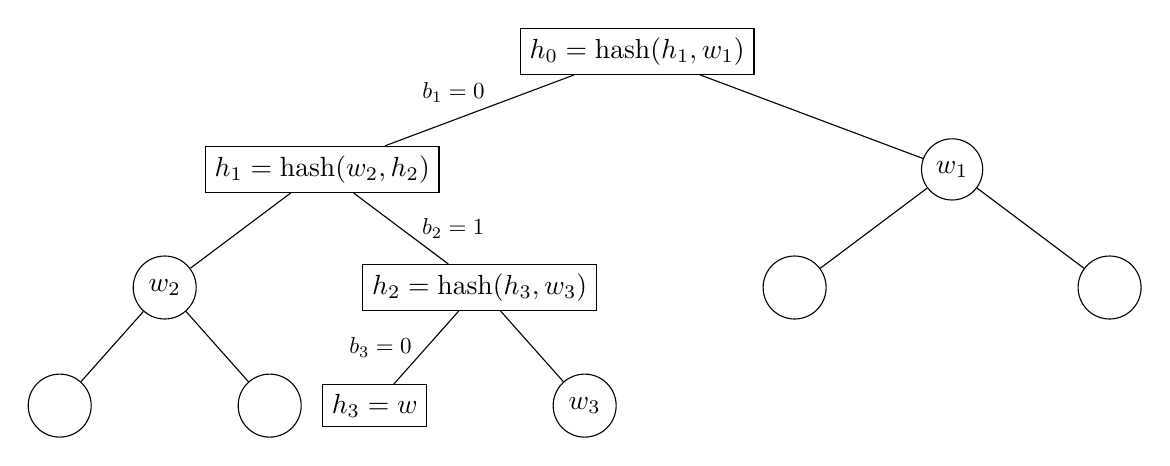
\begin{tikzpicture}[level/.style={sibling distance=8cm/#1}]
\renewcommand{\hash}[1]{\mathrm{hash}({#1})}
\node [rectangle, draw] (c)  {$h_0 = \hash{h_1, w_1}$}
	child { node [rectangle, draw] (l)  {$h_1 = \hash{w_2, h_2}$}  
		child { node [circle, draw, minimum size=0.8cm] (ll) {$w_2$} 
			child { node [circle, draw, minimum size=0.8cm] (lll) {}}
			child { node [circle, draw, minimum size=0.8cm] (llr) {}}
		}
		child { node [rectangle, draw] (B)  {$h_2 = \hash{h_3, w_3}$} 
			child { node [rectangle, draw] (lrl) {$h_3 = w$} 
				edge from parent node[scale=0.83, left=0.1cm] {$b_3= 0$}	
			}
			child { node [circle, draw, minimum size=0.8cm](lrr) {$w_3$}}
			edge from parent node[scale=0.83, right=0.2cm] {$b_2= 1$}	
		}
		edge from parent node[scale=0.83, left=0.4cm, above=0.0cm] {$b_1 = 0$}	
	}
	child { node [circle, draw] (r) {$w_1$}
		child { node [circle, draw, minimum size=0.8cm] (rl) {$$}
		 }
		child { node [circle, draw, minimum size=0.8cm] (rr)  {$$}
		} 
	}
;
\end{tikzpicture}

        \caption{An~example Merkle tree.}
        \label{fig:merkle}
    \end{figure}

    The~above definitions are illustrated in~Figure~\ref{fig:merkle} which~shows a~Merkle tree with~a~distinguished
    node $n = 010$. The~label $w$ of~$n$, together with~labels $w_3$, $w_2$ and~$w_1$, are used to~compute hashes
    $h_3, \,\ldots, \,h_0$.


    Now, going back the~lottery setting, a~Merkle tree for~a~lottery description L is~a~Merkle tree with~minimal height
    such that~for~every $(a_i, R_i, r_i)$ in~$P(L)$ there exists a~leaf labeled with~$hash(a_i, R_i, r_i)$.
    This definition allows many different Merkle trees for~a given $L$, so we assume that~all lottery participants
    agree on~a~common algorithm that~builds a~"canonical" tree $M(L)$ for~each $L$, so that~every payee may construct
    $M(L)$ after receiving $L$. Alternatively, the~sender may send a~tree for~$L$ together with~$L$ to~each payee.
    Note that~the~height of~any Merkle tree for~$L$, that~is~the~maximum depth of~any leaf, is~equal to
    $\text{ceil}(\log_2 P)$.

    A~\textbf{hash of~$L$} is~defined as $h(L) = \hash{\hash{B(L)), h(M(L)}}$, where $B(L)$ is~the~binary encoding of~$L$
    and~$h(M(L))$ is~the~label of~the~root of~$M(L)$.

    A~\textbf{winner certificate} $C = (a, R, r, b_1, \ldots, b_d, w_1, \ldots, w_d)$ consists of
    \begin{itemize}
    \item an Ethereum address $a$ of~the~proposed winner,
    \item S-bit words $R$ and~$r$ encoding respectively the beginning and the length of
      the range within which the S-bit random value must fall,
    \item a~sequence $b_1, \ldots, b_d$ of~bits, with~$d \geq 0$,
    \item a~sequence $w_1, \ldots, w_d$ of~256-bit words.
    \end{itemize}
    %
    Given $C$ we define the sequence $h_d, h_{d-1}, \ldots, h_0$ of 256-bit words as follows:
    \begin{align*}
      h_d    &= \hash{a, R, r} \\
      h_{i-1} &= \begin{cases}
        \hash{h_i, w_i} &\text{if}\ b_i = 0\\
        \hash{w_i, h_i} &\text{if}\ b_i = 1
      \end{cases}
    \end{align*}
    %
    Let $x$ be a~S-bit random value. $C$ is~\textbf{valid} for~$x$ if
    \begin{displaymath}
      R \leq x < R + r  \quad\text{and}\quad \hash{\hash{B(L)}, h_0} = h(L).
    \end{displaymath}
    %
    A Solidity implementation of the algorithm that checks the validity of a winner certificate is
    coded in Appendix~\ref{sec:code} as the function \verb!checkCertificate! with the following signature:
    \begin{quote}
      \verb|function checkCertificate(uint32 rand, bytes32 lotteryHash, bytes32 descriptionHash,|\\
      \verb|                          WinnerCertificate cert) returns (bool)|
    \end{quote}
    The argument \verb|rand| is~the~random value ($x$ in~the~description above, with precision $S = 32$),
    \verb|lotteryHash| is~$\lotteryhash{L}$, \verb|descriptionHash| is~$\hash{B(L)}$ and \verb|cert| is
    a struct encoding a winner certificate.

\section{Contract code}
\label{sec:code}

    It's an~Ethereum contract written in~Solidity. Take into~account that~is~a~simple version of~lottery with~more
    fields in~\texttt{LotteryData} struct for~more clarity.

    \begin{tabularx}{\linewidth}{l}
        \texttt{contract LotteryAgent \{}\\
        \qquad\texttt{uint golem\_dep;  // golem account for~provisions}\\
        \\
        \qquad\texttt{uint constant maturity = 10; // blocks}\\
        \qquad\texttt{uint constant agentMaturity = 28800; // blocks}\\
        \qquad\texttt{uint constant deadline = 86400; // seconds}\\
        \\
        \qquad\texttt{struct LotteryData \{  // in~real-life this struct can fill 2 storage words}\\
        \qquad\qquad\texttt{uint value;}\\
        \qquad\qquad\texttt{uint maturity;}\\
        \qquad\qquad\texttt{uint deadline;}\\
        \qquad\qquad\texttt{uint32 randVal;}\\
        \qquad\qquad\texttt{address payer;}\\
        \qquad\qquad\texttt{address winner;}\\
        \qquad\texttt{\}}\\
        \\
        \qquad\texttt{struct WinnerCertificate \{}\\
        \qquad\qquad\texttt{uint256 uid;        // lottery id}\\
        \qquad\qquad\texttt{address winner;     // winner's address}\\
        \qquad\qquad\texttt{uint32 rangeStart;  // beginning of~the~range}\\
        \qquad\qquad\texttt{uint32 rangeLength; // length of~the~range}\\
        \qquad\qquad\texttt{bool[] path;        // encoding of~the~leaf as a~sequence $b_1, \ldots, b_d$}\\
        \qquad\qquad\texttt{bytes32[] values;   // values $w_1, \ldots, w_d$}\\
        \qquad\texttt{\}}\\
        \\
        \qquad\texttt{mapping (bytes32 => LotteryData) lotteries;}\\
        \\
        \qquad\texttt{function lotteryInit(bytes32 lotteryHash) \{}\\
        \qquad\qquad\texttt{LotteryData lottery = lotteries[lotteryHash];}\\
        \qquad\qquad\texttt{if (lottery.value != 0)}\\
        \qquad\qquad\qquad\texttt{return;}\\
        \qquad\qquad\texttt{uint payerDeposit = countInitPayerDeposit(msg.value);}\\
        \qquad\qquad\texttt{uint value = msg.value - payerDeposit;}\\
        \qquad\qquad\texttt{lotteries[lotteryHash] = LotteryData(value, block.number + maturity, 0, 0,}\\
        \qquad\qquad\qquad\qquad\qquad\qquad\qquad\qquad\qquad\qquad\qquad\qquad\texttt{msg.sender, 0);}\\
        \qquad\texttt{\}}\\
        \\
        \qquad\texttt{function lotteryCaptureHash(bytes32 lotteryHash) \{}\\
        \qquad\qquad\texttt{LotteryData lottery = lotteries[lotteryHash];}\\
        \qquad\qquad\texttt{if (lottery.value == 0)}\\
        \qquad\qquad\qquad\texttt{return;}\\
        \\
        \qquad\qquad\texttt{if (lottery.randVal != 0 )}\\
        \qquad\qquad\qquad\texttt{return;}\\
        \\
        \qquad\qquad\texttt{if (block.number <= lottery.maturity)}\\
        \qquad\qquad\qquad\texttt{return;}\\
        \\
        \qquad\qquad\texttt{if (lottery.maturity + 128 <= block.number)}\\
        \qquad\qquad\qquad\texttt{lottery.payer.send(countPayerDeposit(lottery.value));}\\
        \qquad\qquad\texttt{else if~(lottery.maturity + 256 <= block.number)}\\
        \qquad\qquad\qquad\texttt{msg.sender.send(countPayerDeposit(lottery.value));}\\
        \qquad\qquad\texttt{else}\\
        \qquad\qquad\qquad\texttt{golem\_dep += countPayerDeposit(lottery.value);}\\
        \\
        \qquad\qquad\texttt{lottery.randVal = random(lottery.maturity);}\\
        \qquad\qquad\texttt{lottery.maturity = 0;}\\
        \qquad\qquad\texttt{lottery.payer = 0;}\\
        \qquad\texttt{\}}\\
        \\
        \qquad\texttt{function lotteryWinner(bytes32 lotteryHash) \{}\\
        \qquad\qquad\texttt{LotteryData lottery = lotteries[lotteryHash];}\\
        \qquad\qquad\texttt{if (lottery.value == 0)}\\
        \qquad\qquad\qquad\texttt{return;}\\
        \\
        \qquad\qquad\texttt{if (msg.value < calculateWinnerDeposit(lottery.value))}\\
        \qquad\qquad\qquad\texttt{return;}\\
        \\
        \qquad\qquad\texttt{if (lottery.winner != 0 \&\& block.number <= lottery.maturity)}\\
        \qquad\qquad\qquad\texttt{return;}\\
        \\
        \qquad\qquad\texttt{lottery.winner = msg.sender;}\\
        \qquad\qquad\texttt{lottery.deadline = now + deadline;}\\
        \\
        \qquad\qquad\texttt{if (lottery.randVal == 0) \{}\\
        \qquad\qquad\qquad\texttt{lotteryCaptureHash(lotteryHash);}\\
        \qquad\qquad\texttt{\}}\\
        \qquad\texttt{\}}\\
        \\
        \qquad\texttt{function lotteryPayout(bytes32 lotteryHash) \{}\\
        \qquad\qquad\texttt{LotteryData lottery = lotteries[lotteryHash];}\\
        \qquad\qquad\texttt{if (lottery.winner == 0)}\\
        \qquad\qquad\qquad\texttt{return;}\\
        \qquad\qquad\texttt{if (now <= lottery.deadline)}\\
        \qquad\qquad\qquad\texttt{return;}\\
        \\
        \qquad\qquad\texttt{uint deposit = calculateWinnerDeposit(lottery.value);}\\
        \qquad\qquad\texttt{lottery.winner.send(lottery.value + deposit);}\\
        \qquad\qquad\texttt{delete lotteries[lotteryHash];}\\
        \qquad\texttt{\}}\\
        \\
        \qquad\texttt{function checkCertificate(uint32 rand, bytes32 lotteryHash, WinnerCertificate cert)}\\
        \qquad\qquad\qquad\qquad\qquad\qquad\qquad\qquad\texttt{internal returns (bool) \{}\\
        \qquad\qquad\texttt{// Check if~random val falls into~the~range}\\
        \qquad\qquad\texttt{if (rand < cert.rangeStart $\|$ rand >= cert.rangeStart + cert.rangeLength)}\\
        \qquad\qquad\qquad\texttt{return false;}\\
        \\
        \qquad\qquad\texttt{// Initially, h is~the~value stored in~the~leaf ($h_d$)}\\
        \qquad\qquad\texttt{bytes32 h = bytes32((uint256(cert.winner) * (2 ** 64))}\\
        \qquad\qquad\qquad\qquad\qquad\qquad\texttt{+ (uint256(cert.rangeStart) * (2 ** 32))}\\
        \qquad\qquad\qquad\qquad\qquad\qquad\texttt{+ (cert.rangeLength)}\\
        \qquad\qquad\qquad\qquad\qquad\texttt{);}\\
        \\
        \qquad\qquad\texttt{// Update h with~hashes $h_{d-1}, \ldots, h_0$}\\
        \qquad\qquad\texttt{for (uint i = cert.path.length; i > 0; i--) \{}\\
        \qquad\qquad\qquad\texttt{if (cert.path[i-1] == false)}\\
        \qquad\qquad\qquad\qquad\texttt{h = sha3(h, cert.values[i-1]);}\\
        \qquad\qquad\qquad\texttt{else}\\
        \qquad\qquad\qquad\qquad\texttt{h = sha3(cert.values[i-1], h);}\\
        \qquad\qquad\qquad\texttt{\}}\\
        \qquad\qquad\texttt{// Mix with~uid}\\
        \qquad\qquad\texttt{h = sha3(cert.uid, h);}\\
        \\
        \qquad\qquad\texttt{return h == lotteryHash;}\\
        \qquad\texttt{\}}\\
        \\
        \qquad\texttt{function lotteryCheck(bytes32 lotteryHash, uint256 uid, address winner, uint32 rangeStart,}\\
        \qquad\qquad\qquad\qquad\texttt{uint32 rangeLength, bool[] path, bytes32[] values) \{}\\
        \qquad\qquad\texttt{WinnerCertificate memory winnCert = WinnerCertificate(uid, winner, rangeStart,}\\
        \qquad\qquad\qquad\qquad\qquad\qquad\qquad\texttt{rangeLength, path, values);}\\
        \qquad\qquad\texttt{LotteryData lottery = lotteries[lotteryHash];}\\
        \qquad\qquad\texttt{if (lottery.value == 0 $\|$ block.number <= lottery.maturity)}\\
        \qquad\qquad\qquad\texttt{return;}\\
        \\
        \qquad\qquad\texttt{if (lottery.randVal == 0) \{}\\
        \qquad\qquad\qquad\texttt{lotteryCaptureHash(lotteryHash);}\\
        \qquad\qquad\texttt{\}}\\
        \\
        \qquad\qquad\texttt{if (!checkCertificate(lottery.randVal, lotteryHash, winnCert)) \{}\\
        \qquad\qquad\qquad\texttt{return;}\\
        \qquad\qquad\texttt{\}}\\
        \\
        \qquad\qquad\texttt{if (lottery.winner != 0) \{}\\
        \qquad\qquad\qquad\texttt{if (msg.sender != winner) \{}\\
        \qquad\qquad\qquad\qquad\texttt{msg.sender.send(calculateWinnerDeposit(lottery.value));}\\
        \qquad\qquad\qquad\qquad\texttt{winner.send(lottery.value);}\\
        \qquad\qquad\qquad\texttt{\} else \{}\\
        \qquad\qquad\qquad\qquad\texttt{winner.send(lottery.value + calculateWinnerDeposit(lottery.value));}\\
        \qquad\qquad\qquad\texttt{\}}\\
        \qquad\qquad\texttt{\} else \{}\\
        \qquad\qquad\qquad\texttt{if (msg.sender != winner \&\& block.number > lottery.maturity + agentMaturity) \{}\\
        \qquad\qquad\qquad\qquad\texttt{// Sender is~lottery agent}\\
        \qquad\qquad\qquad\qquad\texttt{msg.sender.send(countAgentCommission(lottery.value));}\\
        \qquad\qquad\qquad\qquad\texttt{winner.send(lottery.value - countAgentCommission(lottery.value));}\\
        \qquad\qquad\qquad\texttt{\} else \{}\\
        \qquad\qquad\qquad\qquad\texttt{winner.send(lottery.value);}\\
        \qquad\qquad\qquad\texttt{\}}\\
        \qquad\qquad\texttt{\}}\\
        \\
        \qquad\qquad\texttt{delete lotteries[lotteryHash];}\\
        \qquad\texttt{\}}\\
        \\
        \qquad\texttt{function changeMaturity(uint maturity) internal constant returns(uint) \{}\\
        \qquad\qquad\texttt{uint begMod = (block.number - 256) \% 256;}\\
        \qquad\qquad\texttt{uint matMod = maturity \% 256;}\\
        \qquad\qquad\texttt{maturity = (block.number - 256) + matMod - begMod;}\\
        \qquad\qquad\texttt{if (begMod > matMod) \{}\\
        \qquad\qquad\qquad\texttt{maturity += 256;}\\
        \qquad\qquad\texttt{\}}\\
        \qquad\qquad\texttt{return maturity;}\\
        \qquad\texttt{\}}\\
        \\
        \qquad\texttt{function random(uint maturity) internal constant returns(uint32) \{}\\
        \qquad\qquad\texttt{if (block.number - maturity > 256)}\\
        \qquad\qquad\qquad\texttt{maturity = changeMaturity(maturity);}\\
        \\
        \qquad\qquad\texttt{return uint32(block.blockhash(maturity));}\\
        \qquad\texttt{\}}\\
        \\
        \qquad\texttt{function calculateWinnerDeposit(uint val) internal constant returns (uint) \{}\\
        \qquad\qquad\texttt{return val / 2;}\\
        \qquad\texttt{\}}\\
        \\
        \qquad\texttt{function countInitPayerDeposit(uint val) internal constant returns (uint) \{}\\
        \qquad\qquad\texttt{return val / 11;}\\
        \qquad\texttt{\}}\\
        \\
        \qquad\texttt{function countPayerDeposit(uint val) internal constant returns (uint) \{}\\
        \qquad\qquad\texttt{return val / 10;}\\
        \qquad\texttt{\}}\\
        \\
        \qquad\texttt{function countAgentCommission(uint val) internal constant returns(uint) \{}\\
        \qquad\qquad\texttt{return val / 10;}\\
        \qquad\texttt{\}}\\
        \\
        \texttt{\}}\\
    \end{tabularx}

\section{Probabilities}

    Let's examine how quickly a~lottery participant can receive her remuneration for~work. For simplicity let's assume
    that~one person always count similar task with~the~same number of~compute users that~do the~same amount of~work
    for~the~same rates. Therefore we can model a~lottery as a~Bernoulli trial. Probability of~success in~this trial is
    equal to~$1/n$ where $n$ is~a~number of~participant. There prize is~equal to~$v$, where one person reward for~a
    task should be $v/n$. Therefore a~participant expects to~receive a~reward after $n$ lotteries.

    The~probability distribution of~the~number of~lotteries before~first winning is~a~geometric distribution with
    $p = 1/n$. Probability that~a~user will have to~take part in~$k$ lotteries before~winning for~a first time is
    equal to
    \begin{displaymath}
	    P(X = k) = \frac{1}{n} \cdot (1 - \frac{1}{n})^{k-1}
	\end{displaymath}

    Therefore probability that~she receive payment before~this time is~above 63\%, the~probability that~she has to~wait
    no longer than $2 \cdot n$ lotteries  is~ above~$86\%$. See figures \ref{fig:geo} and~\ref{fig:geo100} for~details.

    \begin{figure}
        \centering
        \includegraphics[scale=0.6]{geo10.pdf}
        \caption{Plot illustrates what is~a~probability of~waiting $k$ lotteries for~a first pize, when 10 participants
        takes part in~every lottery}
        \label{fig:geo}
    \end{figure}

    \begin{figure}
        \centering
        \includegraphics[scale=0.6]{geo100.pdf}
        \caption{Plot illustrates what is~a~probability of~waiting $k$ lotteries for~a first pize, when
        100 participants take part in~every lottery}
        \label{fig:geo100}
    \end{figure}

    Let's now examine how high is~the~probability of~receiving a~whole earned amount in~a~long run. If~a~user took part
    in~$k$ lotteries, than his expected income should be equal to~$k/n$. We would like to~know what is~a~probability
    of~receiving at~least  80\% of~this value. We can use a~binomial cumulative distribution function for~this.
    The~probability can be described with~a~formula
    \begin{displaymath}
        1 - F((\frac{k}{n})\cdot 80\%, k, \frac{1}{n}) + f((\frac{k}{n})\cdot 80\%, k, \frac{1}{n}))
    \end{displaymath}
    where $f$ is~binomial probability mass function and~$F$ is~binomial cumulative distribution function.

    For 50 lotteries the~probability is~$\sim$75\%  and~for~300 above~$90\%$. See figure \ref{fig:prob} for~details.


    \begin{figure}
        \centering
        \includegraphics[scale=0.6]{prob10.pdf}
        \caption{Plot illustrates what is~a~probability of~receiving at~least 80\% of~expected income after $k$
        lotteries when 10 participants take part in~every lottery}
        \label{fig:prob}
    \end{figure}

\end{document}
